\documentclass[11pt,a4paper]{article}
\usepackage{fontspec}
\setmainfont{DejaVu Sans}[Scale=0.9]
\usepackage{amsmath,amssymb}
\usepackage[left=16mm,right=16mm,top=14mm,bottom=14mm]{geometry}
\usepackage{tabularx,xcolor,array}
\usepackage{graphicx}
\usepackage{tikz}
\definecolor{grau}{gray}{0.42}
\pagestyle{empty}
\setlength{\parindent}{0pt}
\newcommand{\w}[1]{{\small\color{grau}$|$ #1}}
% eine Zeile: links Leistung, rechts Werkzeug
\newcommand{\z}[2][]{\par\noindent #2\hfill\w{#1}\par}
\newcommand{\zz}[1]{\par\noindent #1\par}
\newcommand{\orig}[1]{\clearpage{\small\color{grau}Aufgabenstellung (Original)}\par\vspace{4pt}\begin{center}#1\end{center}\clearpage}

\begin{document}
\orig{\fbox{\includegraphics[page=2,height=0.9\textheight]{fhr26c.pdf}}}

{\large\bfseries 1 Differentialrechnung}\hfill{\small\color{grau}FHR 2026 C · Weg B: amtlicher Erwartungshorizont + 3 Änderungen}\par
\vspace{2pt}\hrule height 1.2pt\vspace{6pt}
{\small $f(x)=-6x^5+18{,}75x^4+20x^3-90x^2$; \ Stellen: $x_E$ Extrem-, $x_W$ Wende-, $x_S$ Sattelstelle}\par\vspace{6pt}

\renewcommand{\arraystretch}{1.25}
\begin{tabularx}{\linewidth}{|c|>{\setlength{\parskip}{3pt}}X|c|}
\hline
\textbf{Teil} & \centering\textbf{Erwartete Teilleistung} (alternative Lösungswege möglich) & \textbf{Pkt.}\\ \hline
1a) &
\zz{Abbildung 3 ist richtig, da}
\z[$f(0)=0$]{\quad • $G_f$ durch den Ursprung verlaufen muss und}
\z[führender Term $-6x^5$]{\quad • $\lim\limits_{x\to-\infty}f(x)=+\infty$ \ und \ $\lim\limits_{x\to+\infty}f(x)=-\infty$}
& 3\\ \hline
1b) &
\z[Symmetrie am Term]{(I): wahr, da es auch gerade Exponenten am $x$ gibt}
\z[$f(x)=x^2\cdot(\ldots)$]{(II): falsch, da es mehr als eine Nullstelle gibt}
\zz{(III): wahr, die Monotonie wechselt zweimal, die Krümmung aber dreimal}
& 3\\ \hline
1c) &
\z[Potenzregel]{$f'(x)=-30x^4+75x^3+60x^2-180x$}
\zz{$f''(x)=-120x^3+225x^2+120x-180$}
\zz{$f'''(x)=-360x^2+450x+120$}
& 3\\ \hline
1d) &
\z[Punktprobe]{Punkt $B$ liegt auf $G_f$, da $f(-2)=-28$.}
\zz{$f'(-2)=-480$}
\z[$t(x)=mx+n$]{$-28=-480\cdot(-2)+n$}
\zz{$t(x)=-480x-988$}
& 3\\ \hline
1e) &
\z[hinreichend: $f''(x_E)\neq0$]{$f'(-1{,}5)=0$; \ $f''(-1{,}5)=551{,}25>0$; \ $f(-1{,}5)\approx-129{,}52$}
\zz{$T(-1{,}5\,|\,{-129{,}52})$ ist ein Tiefpunkt.}
\zz{$f'(0)=0$; \ $f''(0)=-180<0$; \ $f(0)=0$}
\zz{$H(0\,|\,0)$ ist ein Hochpunkt.}
\z[$f''(x_S)=0$, $f'''(x_S)\neq0$]{$f'(2)=0$; \ $f''(2)=0$; \ $f'''(2)=-420\neq0$; \ $f(2)=-92$}
\zz{$S(2\,|\,{-92})$ ist ein Sattelpunkt.}
\vspace{2pt}
\z[Vorzeichen von $f'$]{Monotonieverhalten: \
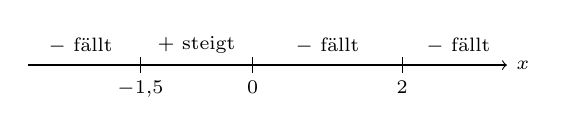
\begin{tikzpicture}[baseline=-3pt,x=0.95cm]
  \draw[->] (-3,0) -- (3.4,0) node[right,font=\scriptsize] {$x$};
  \draw (-1.5,0.1)--(-1.5,-0.1); \node[below,font=\scriptsize] at (-1.5,-0.08) {$-1{,}5$};
  \draw (0,0.1)--(0,-0.1); \node[below,font=\scriptsize] at (0,-0.08) {$0$};
  \draw (2,0.1)--(2,-0.1); \node[below,font=\scriptsize] at (2,-0.08) {$2$};
  \node[above,font=\scriptsize] at (-2.3,0.02) {$-$ fällt};
  \node[above,font=\scriptsize] at (-0.75,0.02) {$+$ steigt};
  \node[above,font=\scriptsize] at (1,0.02) {$-$ fällt};
  \node[above,font=\scriptsize] at (2.75,0.02) {$-$ fällt};
\end{tikzpicture}}
\zz{$-\infty<x<-1{,}5$: \ $G_f$ ist monoton fallend}
\zz{$-1{,}5<x<0$: \ $G_f$ ist monoton steigend}
\zz{$0<x<\infty$: \ $G_f$ ist monoton fallend}
& 8\\ \hline
1f) &
\z[$x=2$ aus 1e) oder Wertetabelle]{$f''(x)=-120x^3+225x^2+120x-180=0$; \ $x_{W1}=2$}
\z[Polynomdivision oder Hornerschema]{$(-120x^3+225x^2+120x-180):(x-2)=-120x^2-15x+90$}
\z[pq-Formel]{$0=x^2+\tfrac18x-\tfrac34$}
\zz{$x_{W2}\approx-0{,}93$; \ $x_{W3}\approx0{,}81$}
\z[hinreichend: $f'''(x_W)\neq0$]{$f'''(-0{,}93)\approx-610{,}7\neq0$; \ $f(-0{,}93)\approx-75{,}83$; \ $W_2(-0{,}93\,|\,{-75{,}83})$}
\zz{$f'''(0{,}81)\approx248{,}9\neq0$; \ $f(0{,}81)\approx-42{,}11$; \ $W_3(0{,}81\,|\,{-42{,}11})$}
\zz{{\small Hinweis: Der Sattelpunkt muss nicht erneut nachgewiesen werden.}}
& 7\\ \hline
 & \hfill Summe & 27\\ \hline
\end{tabularx}
\end{document}
